\chapter{Neutron Star Equation of State}
\label{chap:chapter-2}

In this chapter, we take a heuristic approach in building up to the rather complex modern prescriptions of neutron star structure. 
Astrophysicists have posited still-relevant models of stellar structure before the frameworks of general relativity and quantum mechanics were even known, mostly forming their understanding fundamentally with thermodynamical and statistical arguments and an as-yet unchallenged Newtonian description of gravity.
This plan is also used in hindsight.
As a description of a system gets more complicated (finite-temperature nuclear physics, indirect extrapolations of observational and experimental data), it is often necessary to ground our understanding with an approximate model.
Here, the simple model for the equation of state is that of a polytrope, or one where the pressure is only dependent on the density of the fluid or gas:
\begin{align}
P(\rho_0) = K \rho_0^\Gamma = (\Gamma -  1) \rho_0 \epsilon,
\end{align}
where $P$ is pressure, $\epsilon$ specific internal energy, $\rho_0$ rest-mass density, $K$ the polytropic constant, and $\Gamma$ is a unitless exponent often referred to as the adiabatic index.
Since the density only varies with the pressure, this model assumes the fluid is barotropic.

This simple model reveals itself to be important in limiting cases of stellar matter.  
For a high-mass neutron star where the average density is well above the nuclear saturation number density $n_s$, the star can be roughly approximated with a $\Gamma \approx 2$ polytrope~\cite{lattimer2016equation}.  
At low densities, where the average density is well below $n_s$, the star is mostly supported by degenerate relativistic Fermi pressure (as in the high-mass white dwarf model) such that $\Gamma \simeq 4/3$.
Introducing the notion that the interior region of the star may have a different adiabatic index to the crust, and that the core could be composed of exotic matter, a more adaptable equation of state can be constructed with a set of polytropes each defining these regions.  
These equations of state are called piecewise-polytropes.  

However, the polytrope models do not adequately account for effects of temperature or composition variation of our very dense fluid matter.  
So called ``hot'' or finite-temperature equations of state are much more general, and generally constructed as multivariable tables utilizing many constraints from nuclear theory, astrophysics observations, and particle experiments.
Because of the complexities for codes to utilize these equations of state, piecewise-polytropes are often used as a way to curve-fit and cheat the incorporation of temperature in their routines, as well as to provide a simple method to tune parameters of the PP to explore a wide range of neutron star compactnesses.
In addition, an effective adiabatic index can be extracted to give one a sense how stiff the structure is in a given density regime:
\begin{align}
\label{e:adiabat}
\tilde{\Gamma} \equiv \left( \frac{d\, {\rm log} P}{d\, {\rm log} \rho_0} \right) _S
\end{align}

First, we'll review the theory of polytrope based models in Section \ref{sec:polytropes}. Then we will outline the many experimental, observational and nuclear theory constraints on the equation of state in Section \ref{sec:constraints}.   In Section \ref{sec:nuclear-eos}, we include a description of the microphysical equations of state used in the simulations of Chapter \ref{chap:chapter-5}. 


\section{Polytrope-based models}
\label{sec:polytropes}

Neutron stars in early simulations were initially modeled with the polytrope, or ``Gamma-Law'', equation of state, in the range where $2 < \Gamma < 3$.
For higher $\Gamma$'s, the gas pressure is stronger, and we often refer to these as ``stiff'' equations of state and look poofier, or less compact.
Conversely, stars with smaller $\Gamma$'s are called ``soft''.  Soft equations of state are hence more compact.

We do not expect, further, that the core, interior or crust to all have the same polytropic description.
In that case, the Gamma-Law description of neutron star structure can be improved by a so-called piecewise polytrope model.
In such models, we allow each specified dnesity interval to have its own equation of state such that 
$$P(\rho_0) = K_i \rho_0^{\Gamma_i}$$
where the adiabatic index $\Gamma_i$ is a constant in between each density interval (defined by a set of dividing-densities $\{\rho_1,\rho_2,...,\rho_{i-1} \}$), and $K_i$ is chosen so that the equation of state is continuous across interfaces.
Piecewise polytropes, while multi-parameter, are still single-variable descriptions of stellar structure.  
A first method of adding thermal dependencies to any polytrope model is to augment the ``cold'' equation of state:
\begin{align}
P &=  P_{\rm cold}(\rho_0) + (\Gamma_{\rm th}-1)\rho\epsilon_{\rm th} ,\\
\epsilon &=  \epsilon_{\rm cold}(\rho_0) + \epsilon_{\rm th}, 
\end{align}
where $\epsilon_{\rm th}$ is a thermal specific energy, which is determined during the evolution of the energy density.
In~\cite{read2009constraints}, a systematic study of parametrizing the constraints of the neutron star equation of state  with piecewise polytrope models was studied.  
Phenomenologically different piecewise polytrope models yielded different tidal deformability parameters, which was detectable in the gravitational wave signal.


In addition to the density dependence of pressure, a more realistic equation of state has to include dependence on temperature, $T$, and composition, for instance the fraction of electrons per baryons $Y_e = n_e / n_b$.  
We expect the temperature to be a factor, since hydrodynamical shocks heat the system, and the composition to vary due to charged-current weak nuclear processes that may be on the timescales of the merger time, and neutrinos allow for cooling or further heating via neutrino emission and absorption. 
In general, this equation of state system takes the form:
\begin{align}
P &= P(\rho_0, T, X_i), \\
u &= u(\rho_0, T, X_i),
\end{align}
where $X_i$ can be any number of composition variables.  
Note that in nuclear statistical equilibrium (NSE), as in our models, the only composition variable is the electron fraction, $Y_e$.  
NSE only breaks down in the ejecta, only after the fluid has decompressed considerably.

\section{Neutron Star Constraints}
\label{sec:constraints}

Results from X-ray binary observations constrain the areal radius of $1.4M_\odot$ neutron stars between $10.4 - 12.9 \textrm{km}$, using X-ray bursts to obtain both the mass and radius simultaneously~\cite{van1979possible,ozel2006soft}.
Observations from the neutron star-white dwarf binary PSR J1614-2230~\cite{ozel2010massive} revealed a neutron star mass $1.97 \pm 0.04 M_\odot$, and later measurements from PSR J0348+0432~\cite{antoniadis2013massive} showed masses slightly higher at  $2.01 \pm 0.04 M_\odot$.  Therefore, an equation of state must allow for a maximal mass of $\sym 2 M_{\odot}$.
The most rapidly spinning pulsar PSR J1748-2446ad~\cite{hessels2006radio} constrains the maximum radius of a neutron star: a star must rotate beneath the Keplerian frequency at which mass-shedding occurs (cf. Equation [95] in~\cite{lattimer2016equation}).
Lower bounds on the neutron star radius can be obtained through causality, namely that the sound speed $c_s^2 \equiv c^2 \partial p / \partial \epsilon$ must not be superluminal (i.e. $c_s^2 \le c^2$), which gives bounds on the maximal neutron star compaction, or larger minimum radii~\cite{Haensel:1999}.

The equations of state discussed in the next few sections all satisfy that the observational constraint that $M_{\rm NS} \gtrsim 2 M_\odot$.
The radii of their $1.2 M_\odot$ neutron stars are also in the most likely range provided by studies supported by nuclear theory and X-ray binary observations~\cite{Steiner2010,2013ApJ...765L...5S}, although a separate study of the same astronomical data suggests smaller radii~\cite{Guillot:2013wu}.  
That argument is also  applied in~\cite{steiner2013core} (the foundation of one of the models used in our study), where they modeled their equation of state to give radii closer to this range, $R_{\rm NS} \sim (11-12.5) {\rm km}$, to give slightly more compact stars.

\section{Hot, Microphysical Equations of State}
\label{sec:nuclear-eos}

\subsection{LS220}
\label{sec:ls220}

One of the first finite-temperature equations of state developed for astrophysical simulations is the Lattimer-Swesty (LS) model~\cite{Lattimer:1991nc}.  
For this reason, computationally expensive full, three-dimensional fluid evolutions of core-collapse supernova have only been performed for LS220 and STOS~\cite{Marek2009}.
LS is based on a compressible liquid drop model, using a first-order phase transition from low-density vapor to the high-density liquid phase.  
This makes the density dependence of the transition isobaric.  
The incompressibility parameter is $K_0 = 220 {\rm MeV}$, which is a measure of the incompressibility of nuclear matter, while the symmetry energy is $S_\nu = 29.3$MeV, which represents the binding enregy of symmetric nuclear matter.
This equation of state is argued to be no longer compatible with recent results~\cite{Fischer2014}, based on results from Chiral Effective Field Theory (EFT) that constrain the equation of state at low densities.

\subsection{DD2}
\label{sec:dd2}

Another hot, composition dependent nuclear-theory based equation of state is DD2~\cite{typel2010composition}.  DD2 is relativistic mean field (RMF) model based on a nucleon-meson coupling model whose momentum is density-dependent (DD).  
For DD, the coupling parameters in the model are set by the saturation density (when nucleons begin to touch) of symmetric nuclear matter (i.e. the number densities $n_\textrm{p} = n_\textrm{n}$), where the incompressibility factor is fixed at $K_0 = 240$ MeV~\cite{typel2005relativistic}.
In this model, the binding energy of eight nuclei were computed and compared to experimental values and found stronger agreement than other earlier EOS models.
DD2 is the same as DD~\cite{typel2005relativistic} with additional corrections provided from experimental nucleon masses measured in a lab, with incompressibility $K_0 = 243$MeV and symmetry energy $S_\nu=31.67$MeV.

DD2 is also constrained by several nuclear theory based studies~\cite{hempel2012new}.
Several studies have shown that nuclear energy bounds fall within the predictions of Chiral EFT, which constrains the equation of state in the sub-saturation density regime, so that the free parameters in the DD2 equation of state are constrained by those predictions. 
Unlike the classical Lattimer-Swesty~\cite{Lattimer:1991nc} and the STOS ~\cite{Shen:1998gq} EOS models that employ a single nucleus approximation, DD2 includes a detailed distribution of thousands of different nuclei.
In addition, DD2 allows for the existence of stars whose masses are above the observations we have to-date.
Compared to observational constraints, DD2 can allow for masses as high as $\sym 2.4 M_\odot$, much greater than the observed $\sym 2 M_\odot$ neutron stars.
DD2, however, comes within $\sym 1 \textrm{km}$ of measured areal radii--being just slightly outside with $13.22 \textrm{km}$.

\subsection{FSU2.1}
\label{sec:fsu21}

Another relativistic mean field equation of state is one based on the FSUGold model~\cite{todd2005neutron} with modifications in the high density bins to allow for a maximal neutron star mass of $2.1 M_\odot$~\cite{shen2011second}.  The RMF effective interaction FSUGold model only predicts a $1.7 M_\odot$ maximum mass, and was constructed before the detection of the $1.97 \pm 0.04 M_\odot$ neutron star.
Among the assumptions and constraints that went into the FSUGold equation of state, FSU2.1 removes the restriction that the pressure is independent of proton fraction, and likewise independent of the temperature, as matter is degenerate at high densities.

The upper limit on the baryon number density $n_B$ was modified from $10^{0.4} {\rm fm^{-3}}$ to $10^{0.2} {\rm fm^{-3}}$ for finite temperatures $T \in [10^{-0.8} , 10^{1.875}]\, {\rm MeV}$.  The lower limit is the same as FSU1.7 at $10^{-8.0} {\rm fm^{-3}}$.  For zero-temperature, the proton fraction $Y_p$ is held at $0$ while in the finite-temperature regime, $Y_p \in [0.05 , 0.56]$.  The incompressibility parameter is $K_0 = 230.0 MeV$, constrained by giant resonance of nuclei, while the symmetry energy $S_\nu = 32.59$MeV is constrained by neutron skin thickness of $^208$Pb~\cite{fattoyev2010relativistic}.

\subsection{SFHo and SFHx}
\label{sec:sfh}

Two additional systems were developed by Steiner, Hempel and Fischer~\cite{steiner2013core} that yielded much more compact stars.
In these models, the theoretical constraint enforcing subluminal sound speeds is automatically enforced.  The region where the $M-R$ curve of a $1.4 M_\odot$ neutron star is constrained to lie $R_{\rm NS} \in [11.2,12.3] {\rm km}$ is shown in~\cite{steiner6871apjl}.
The baseline model, SFHo, fits this prediction.  The extreme model, SFHx, attempts to minimize the radius of lower mass neutron stars.  In either case, the pressure monotonically increases with density in all phases.
The incompressibility factor is $K_0 = 245.4$MeV with symmetry energy $S_\nu = 31.57$MeV for SFHo, while $K_0 = 238.8$MeV and $S_\nu = 28.67$MeV for SFHx.

\section{Our survey}

In our survey, we use the Hempel's DD2, Fisher's FSU2.1, and the SFHo and SFHx equations of state.  
LS220 may occasionally be used as a reference. 
In Figure \ref{fig:MvsR}, we show the neutron star mass-radius relationship for each system used in this study. 
We chose to study two neutron star masses, $M_{\rm NS} = (1.2, 1.4) M_{\odot}$, since the distribution of neutron star populations is expected to have a mean in this range. 
In addition, the LS220 equation of state is included, as it has already been simulated in~\cite{Foucart:2014nda}.  
For the initial configuration of the star in isolation, we take a cold, $\beta$-equilibrium slice of three-dimensional equation of state tables.  
To avoid strange artifacts at the table minimum of $T_{\rm floor} = 0.01 {\rm MeV}$, we take a cold slice of  $T = 0.1 {\rm MeV}$.  Therefore, the effective (cold, $\beta$-equilibrium) equation of state table is barotropic. Once the star begins to tidally disrupt, we are no longer in $\beta$-equilibrium.

In~\cite{lattimer2016equation}, Lattimer discusses the number of constraints on the equation of state and how they relate to the mass-radius relations in various ``zones'' of Figure \ref{fig:MvsR}.  
Principally, an equation of state must not allow for superluminal sound speeds and allow for a maximum mass of $\sym 2.1 M_{\odot}$.

\begin{figure}
	\centering
	% GNUPLOT: LaTeX picture with Postscript
\begingroup
\newcommand{\ft}[0]{\footnotesize}
  \makeatletter
  \providecommand\color[2][]{%
    \GenericError{(gnuplot) \space\space\space\@spaces}{%
      Package color not loaded in conjunction with
      terminal option `colourtext'%
    }{See the gnuplot documentation for explanation.%
    }{Either use 'blacktext' in gnuplot or load the package
      color.sty in LaTeX.}%
    \renewcommand\color[2][]{}%
  }%
  \providecommand\includegraphics[2][]{%
    \GenericError{(gnuplot) \space\space\space\@spaces}{%
      Package graphicx or graphics not loaded%
    }{See the gnuplot documentation for explanation.%
    }{The gnuplot epslatex terminal needs graphicx.sty or graphics.sty.}%
    \renewcommand\includegraphics[2][]{}%
  }%
  \providecommand\rotatebox[2]{#2}%
  \@ifundefined{ifGPcolor}{%
    \newif\ifGPcolor
    \GPcolortrue
  }{}%
  \@ifundefined{ifGPblacktext}{%
    \newif\ifGPblacktext
    \GPblacktexttrue
  }{}%
  % define a \g@addto@macro without @ in the name:
  \let\gplgaddtomacro\g@addto@macro
  % define empty templates for all commands taking text:
  \gdef\gplbacktext{}%
  \gdef\gplfronttext{}%
  \makeatother
  \ifGPblacktext
    % no textcolor at all
    \def\colorrgb#1{}%
    \def\colorgray#1{}%
  \else
    % gray or color?
    \ifGPcolor
      \def\colorrgb#1{\color[rgb]{#1}}%
      \def\colorgray#1{\color[gray]{#1}}%
      \expandafter\def\csname LTw\endcsname{\color{white}}%
      \expandafter\def\csname LTb\endcsname{\color{black}}%
      \expandafter\def\csname LTa\endcsname{\color{black}}%
      \expandafter\def\csname LT0\endcsname{\color[rgb]{1,0,0}}%
      \expandafter\def\csname LT1\endcsname{\color[rgb]{0,1,0}}%
      \expandafter\def\csname LT2\endcsname{\color[rgb]{0,0,1}}%
      \expandafter\def\csname LT3\endcsname{\color[rgb]{1,0,1}}%
      \expandafter\def\csname LT4\endcsname{\color[rgb]{0,1,1}}%
      \expandafter\def\csname LT5\endcsname{\color[rgb]{1,1,0}}%
      \expandafter\def\csname LT6\endcsname{\color[rgb]{0,0,0}}%
      \expandafter\def\csname LT7\endcsname{\color[rgb]{1,0.3,0}}%
      \expandafter\def\csname LT8\endcsname{\color[rgb]{0.5,0.5,0.5}}%
    \else
      % gray
      \def\colorrgb#1{\color{black}}%
      \def\colorgray#1{\color[gray]{#1}}%
      \expandafter\def\csname LTw\endcsname{\color{white}}%
      \expandafter\def\csname LTb\endcsname{\color{black}}%
      \expandafter\def\csname LTa\endcsname{\color{black}}%
      \expandafter\def\csname LT0\endcsname{\color{black}}%
      \expandafter\def\csname LT1\endcsname{\color{black}}%
      \expandafter\def\csname LT2\endcsname{\color{black}}%
      \expandafter\def\csname LT3\endcsname{\color{black}}%
      \expandafter\def\csname LT4\endcsname{\color{black}}%
      \expandafter\def\csname LT5\endcsname{\color{black}}%
      \expandafter\def\csname LT6\endcsname{\color{black}}%
      \expandafter\def\csname LT7\endcsname{\color{black}}%
      \expandafter\def\csname LT8\endcsname{\color{black}}%
    \fi
  \fi
  \setlength{\unitlength}{0.0500bp}%
  \begin{picture}(7200.00,5040.00)%
    \gplgaddtomacro\gplbacktext{%
      \csname LTb\endcsname%
      \put(946,704){\makebox(0,0)[r]{\strut{} 0}}%
      \put(946,1518){\makebox(0,0)[r]{\strut{} 0.5}}%
      \put(946,2332){\makebox(0,0)[r]{\strut{} 1}}%
      \put(946,3147){\makebox(0,0)[r]{\strut{} 1.5}}%
      \put(946,3961){\makebox(0,0)[r]{\strut{} 2}}%
      \put(946,4775){\makebox(0,0)[r]{\strut{} 2.5}}%
      \put(1078,484){\makebox(0,0){\strut{} 10}}%
      \put(2032,484){\makebox(0,0){\strut{} 11}}%
      \put(2986,484){\makebox(0,0){\strut{} 12}}%
      \put(3941,484){\makebox(0,0){\strut{} 13}}%
      \put(4895,484){\makebox(0,0){\strut{} 14}}%
      \put(5849,484){\makebox(0,0){\strut{} 15}}%
      \put(6803,484){\makebox(0,0){\strut{} 16}}%
      \put(176,2739){\rotatebox{-270}{\makebox(0,0){\strut{}Gravitational Mass ($M_{\odot}$)}}}%
      \put(3940,154){\makebox(0,0){\strut{}Areal Radius (km)}}%
    }%
    \gplgaddtomacro\gplfronttext{%
      \csname LTb\endcsname%
      \put(5816,4602){\makebox(0,0)[r]{\strut{}Hempel DD2}}%
      \csname LTb\endcsname%
      \put(5816,4382){\makebox(0,0)[r]{\strut{}G. Shen FSU 2.1}}%
      \csname LTb\endcsname%
      \put(5816,4162){\makebox(0,0)[r]{\strut{}SFHo}}%
      \csname LTb\endcsname%
      \put(5816,3942){\makebox(0,0)[r]{\strut{}SFHx}}%
      \csname LTb\endcsname%
      \put(5816,3722){\makebox(0,0)[r]{\strut{}LS220}}%
    }%
    \gplbacktext
    \put(0,0){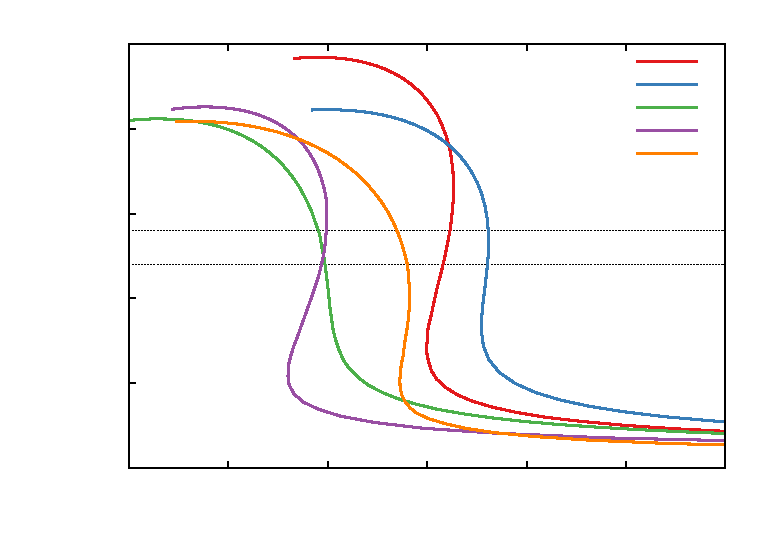
\includegraphics{images/tov-mass-vs-radius}}%
    \gplfronttext
  \end{picture}%
\endgroup

	\caption[Neutron star mass vs. areal radius]{
		ADM neutron star mass vs. areal radius for nuclear equations of state sliced at $T=0.1{\rm MeV}$ in $\beta$-equilibrium.  Intersections of dotted lines and colored curves represent ADM the neutron star masses chosen for this survey: $M_{\rm NS} = (1.2, 1.4) M_{\odot}$.  
	}
	\label{fig:MvsR}
\end{figure}

From the $M-R$ curves in Figure \ref{fig:MvsR} alone, there are a bounty of astrophysics questions we can ask.  
By adopting these finite-temperature, composition-dependent equation of state models for our neutron stars, what observable characterisitics are observed during inspiral and merger?  
How much does the creation of r-process elements in the dynamical outflows vary?  
Does the generated gravitational waveform vary aside from its dependence on the compactness parameter?  
Are the predictions of the fitting formulae~\cite{foucart2012black,pannarale2014black,kawaguchi2016models} of the resulting remnant and ejecta masses correct, even though they were formed with barotropic equations of state?

\begin{figure}
	\centering
	% GNUPLOT: LaTeX picture with Postscript
\begingroup
\newcommand{\ft}[0]{\footnotesize}
  \makeatletter
  \providecommand\color[2][]{%
    \GenericError{(gnuplot) \space\space\space\@spaces}{%
      Package color not loaded in conjunction with
      terminal option `colourtext'%
    }{See the gnuplot documentation for explanation.%
    }{Either use 'blacktext' in gnuplot or load the package
      color.sty in LaTeX.}%
    \renewcommand\color[2][]{}%
  }%
  \providecommand\includegraphics[2][]{%
    \GenericError{(gnuplot) \space\space\space\@spaces}{%
      Package graphicx or graphics not loaded%
    }{See the gnuplot documentation for explanation.%
    }{The gnuplot epslatex terminal needs graphicx.sty or graphics.sty.}%
    \renewcommand\includegraphics[2][]{}%
  }%
  \providecommand\rotatebox[2]{#2}%
  \@ifundefined{ifGPcolor}{%
    \newif\ifGPcolor
    \GPcolortrue
  }{}%
  \@ifundefined{ifGPblacktext}{%
    \newif\ifGPblacktext
    \GPblacktexttrue
  }{}%
  % define a \g@addto@macro without @ in the name:
  \let\gplgaddtomacro\g@addto@macro
  % define empty templates for all commands taking text:
  \gdef\gplbacktext{}%
  \gdef\gplfronttext{}%
  \makeatother
  \ifGPblacktext
    % no textcolor at all
    \def\colorrgb#1{}%
    \def\colorgray#1{}%
  \else
    % gray or color?
    \ifGPcolor
      \def\colorrgb#1{\color[rgb]{#1}}%
      \def\colorgray#1{\color[gray]{#1}}%
      \expandafter\def\csname LTw\endcsname{\color{white}}%
      \expandafter\def\csname LTb\endcsname{\color{black}}%
      \expandafter\def\csname LTa\endcsname{\color{black}}%
      \expandafter\def\csname LT0\endcsname{\color[rgb]{1,0,0}}%
      \expandafter\def\csname LT1\endcsname{\color[rgb]{0,1,0}}%
      \expandafter\def\csname LT2\endcsname{\color[rgb]{0,0,1}}%
      \expandafter\def\csname LT3\endcsname{\color[rgb]{1,0,1}}%
      \expandafter\def\csname LT4\endcsname{\color[rgb]{0,1,1}}%
      \expandafter\def\csname LT5\endcsname{\color[rgb]{1,1,0}}%
      \expandafter\def\csname LT6\endcsname{\color[rgb]{0,0,0}}%
      \expandafter\def\csname LT7\endcsname{\color[rgb]{1,0.3,0}}%
      \expandafter\def\csname LT8\endcsname{\color[rgb]{0.5,0.5,0.5}}%
    \else
      % gray
      \def\colorrgb#1{\color{black}}%
      \def\colorgray#1{\color[gray]{#1}}%
      \expandafter\def\csname LTw\endcsname{\color{white}}%
      \expandafter\def\csname LTb\endcsname{\color{black}}%
      \expandafter\def\csname LTa\endcsname{\color{black}}%
      \expandafter\def\csname LT0\endcsname{\color{black}}%
      \expandafter\def\csname LT1\endcsname{\color{black}}%
      \expandafter\def\csname LT2\endcsname{\color{black}}%
      \expandafter\def\csname LT3\endcsname{\color{black}}%
      \expandafter\def\csname LT4\endcsname{\color{black}}%
      \expandafter\def\csname LT5\endcsname{\color{black}}%
      \expandafter\def\csname LT6\endcsname{\color{black}}%
      \expandafter\def\csname LT7\endcsname{\color{black}}%
      \expandafter\def\csname LT8\endcsname{\color{black}}%
    \fi
  \fi
  \setlength{\unitlength}{0.0500bp}%
  \begin{picture}(7200.00,5040.00)%
    \gplgaddtomacro\gplbacktext{%
      \csname LTb\endcsname%
      \put(1210,820){\makebox(0,0)[r]{\strut{} 1e+27}}%
      \put(1210,1272){\makebox(0,0)[r]{\strut{} 1e+28}}%
      \put(1210,1724){\makebox(0,0)[r]{\strut{} 1e+29}}%
      \put(1210,2177){\makebox(0,0)[r]{\strut{} 1e+30}}%
      \put(1210,2629){\makebox(0,0)[r]{\strut{} 1e+31}}%
      \put(1210,3081){\makebox(0,0)[r]{\strut{} 1e+32}}%
      \put(1210,3534){\makebox(0,0)[r]{\strut{} 1e+33}}%
      \put(1210,3986){\makebox(0,0)[r]{\strut{} 1e+34}}%
      \put(1210,4438){\makebox(0,0)[r]{\strut{} 1e+35}}%
      \put(1571,484){\makebox(0,0){\strut{} 1e+11}}%
      \put(2663,484){\makebox(0,0){\strut{} 1e+12}}%
      \put(3755,484){\makebox(0,0){\strut{} 1e+13}}%
      \put(4847,484){\makebox(0,0){\strut{} 1e+14}}%
      \put(5939,484){\makebox(0,0){\strut{} 1e+15}}%
      \put(176,2739){\rotatebox{-270}{\makebox(0,0){\strut{}Pressure (barye)}}}%
      \put(4072,154){\makebox(0,0){\strut{}Density (g/cm$^3$)}}%
    }%
    \gplgaddtomacro\gplfronttext{%
      \csname LTb\endcsname%
      \put(2329,4602){\makebox(0,0)[l]{\strut{}Hempel DD2}}%
      \csname LTb\endcsname%
      \put(2329,4382){\makebox(0,0)[l]{\strut{}G. Shen FSU 2.1}}%
      \csname LTb\endcsname%
      \put(2329,4162){\makebox(0,0)[l]{\strut{}SFHo}}%
      \csname LTb\endcsname%
      \put(2329,3942){\makebox(0,0)[l]{\strut{}SFHx}}%
      \csname LTb\endcsname%
      \put(2329,3722){\makebox(0,0)[l]{\strut{}LS220}}%
    }%
    \gplbacktext
    \put(0,0){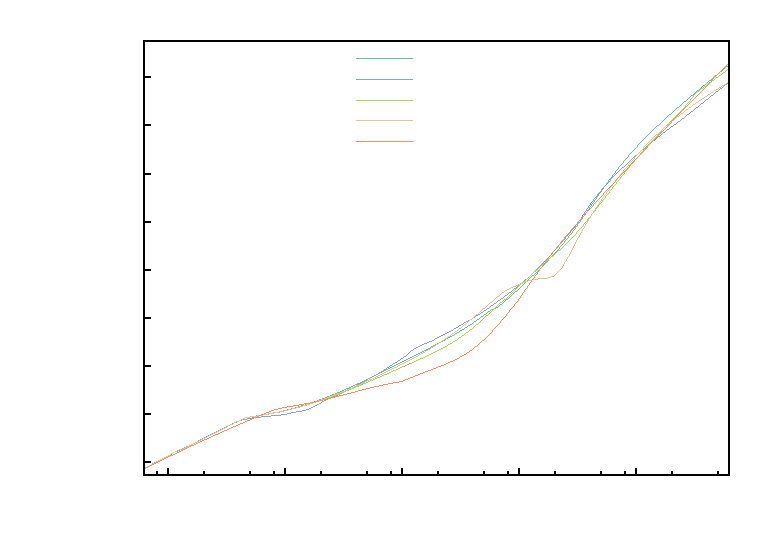
\includegraphics{images/pressure-vs-density}}%
    \gplfronttext
  \end{picture}%
\endgroup

	\caption[Pressure vs. density for a cold, beta-equilibrium slice]{
		Pressure vs. density for finite-temperature, nuclear equations of state used in this study. The initial fluid is chosen to be cold and in $\beta$-equilibrium: $T=0.1 {\rm MeV}$ and $Y_e = Y_e (n_b)$, respectively.  Vertical dotted line represents the fiducial density.
	}
	\label{fig:PvsRho}
\end{figure}

In Figure \ref{fig:PvsRho}, it can be seen that the relationship between pressure and density at low densities is similar to a $\Gamma \approx 2$ polytrope in the ``cold'' regime of the table.  
Qualitatively, the pressure support at lower densities can be stronger for one equation of state, but softer at higher densities compared to another.  
Indeed, it was noted in~\cite{steiner2013core} that the concept of describing an equation of state as stiff or soft can be somewhat misleading.  
That is, the effective adiabatic index $\tilde{\Gamma}$ of Equation \ref{e:adiabat} for the poofier FSU2.1 model is smaller (larger) in the lower (higher) density regions compared to the more compact SFHo in the ``cold'' phase.

%\begin{figure}
%	\centering
%	% GNUPLOT: LaTeX picture with Postscript
\begingroup
  \makeatletter
  \providecommand\color[2][]{%
    \GenericError{(gnuplot) \space\space\space\@spaces}{%
      Package color not loaded in conjunction with
      terminal option `colourtext'%
    }{See the gnuplot documentation for explanation.%
    }{Either use 'blacktext' in gnuplot or load the package
      color.sty in LaTeX.}%
    \renewcommand\color[2][]{}%
  }%
  \providecommand\includegraphics[2][]{%
    \GenericError{(gnuplot) \space\space\space\@spaces}{%
      Package graphicx or graphics not loaded%
    }{See the gnuplot documentation for explanation.%
    }{The gnuplot epslatex terminal needs graphicx.sty or graphics.sty.}%
    \renewcommand\includegraphics[2][]{}%
  }%
  \providecommand\rotatebox[2]{#2}%
  \@ifundefined{ifGPcolor}{%
    \newif\ifGPcolor
    \GPcolortrue
  }{}%
  \@ifundefined{ifGPblacktext}{%
    \newif\ifGPblacktext
    \GPblacktexttrue
  }{}%
  % define a \g@addto@macro without @ in the name:
  \let\gplgaddtomacro\g@addto@macro
  % define empty templates for all commands taking text:
  \gdef\gplbacktext{}%
  \gdef\gplfronttext{}%
  \makeatother
  \ifGPblacktext
    % no textcolor at all
    \def\colorrgb#1{}%
    \def\colorgray#1{}%
  \else
    % gray or color?
    \ifGPcolor
      \def\colorrgb#1{\color[rgb]{#1}}%
      \def\colorgray#1{\color[gray]{#1}}%
      \expandafter\def\csname LTw\endcsname{\color{white}}%
      \expandafter\def\csname LTb\endcsname{\color{black}}%
      \expandafter\def\csname LTa\endcsname{\color{black}}%
      \expandafter\def\csname LT0\endcsname{\color[rgb]{1,0,0}}%
      \expandafter\def\csname LT1\endcsname{\color[rgb]{0,1,0}}%
      \expandafter\def\csname LT2\endcsname{\color[rgb]{0,0,1}}%
      \expandafter\def\csname LT3\endcsname{\color[rgb]{1,0,1}}%
      \expandafter\def\csname LT4\endcsname{\color[rgb]{0,1,1}}%
      \expandafter\def\csname LT5\endcsname{\color[rgb]{1,1,0}}%
      \expandafter\def\csname LT6\endcsname{\color[rgb]{0,0,0}}%
      \expandafter\def\csname LT7\endcsname{\color[rgb]{1,0.3,0}}%
      \expandafter\def\csname LT8\endcsname{\color[rgb]{0.5,0.5,0.5}}%
    \else
      % gray
      \def\colorrgb#1{\color{black}}%
      \def\colorgray#1{\color[gray]{#1}}%
      \expandafter\def\csname LTw\endcsname{\color{white}}%
      \expandafter\def\csname LTb\endcsname{\color{black}}%
      \expandafter\def\csname LTa\endcsname{\color{black}}%
      \expandafter\def\csname LT0\endcsname{\color{black}}%
      \expandafter\def\csname LT1\endcsname{\color{black}}%
      \expandafter\def\csname LT2\endcsname{\color{black}}%
      \expandafter\def\csname LT3\endcsname{\color{black}}%
      \expandafter\def\csname LT4\endcsname{\color{black}}%
      \expandafter\def\csname LT5\endcsname{\color{black}}%
      \expandafter\def\csname LT6\endcsname{\color{black}}%
      \expandafter\def\csname LT7\endcsname{\color{black}}%
      \expandafter\def\csname LT8\endcsname{\color{black}}%
    \fi
  \fi
  \setlength{\unitlength}{0.0500bp}%
  \begin{picture}(7200.00,5040.00)%
    \gplgaddtomacro\gplbacktext{%
      \csname LTb\endcsname%
      \put(946,704){\makebox(0,0)[r]{\strut{} 0}}%
      \put(946,1111){\makebox(0,0)[r]{\strut{} 0.1}}%
      \put(946,1518){\makebox(0,0)[r]{\strut{} 0.2}}%
      \put(946,1925){\makebox(0,0)[r]{\strut{} 0.3}}%
      \put(946,2332){\makebox(0,0)[r]{\strut{} 0.4}}%
      \put(946,2739){\makebox(0,0)[r]{\strut{} 0.5}}%
      \put(946,3147){\makebox(0,0)[r]{\strut{} 0.6}}%
      \put(946,3554){\makebox(0,0)[r]{\strut{} 0.7}}%
      \put(946,3961){\makebox(0,0)[r]{\strut{} 0.8}}%
      \put(946,4368){\makebox(0,0)[r]{\strut{} 0.9}}%
      \put(946,4775){\makebox(0,0)[r]{\strut{} 1}}%
      \put(1318,484){\makebox(0,0){\strut{} 1e+11}}%
      \put(2463,484){\makebox(0,0){\strut{} 1e+12}}%
      \put(3608,484){\makebox(0,0){\strut{} 1e+13}}%
      \put(4753,484){\makebox(0,0){\strut{} 1e+14}}%
      \put(5898,484){\makebox(0,0){\strut{} 1e+15}}%
      \put(176,2739){\rotatebox{-270}{\makebox(0,0){\strut{}$[P(T) - P(0)]/P(T)$}}}%
      \put(3940,154){\makebox(0,0){\strut{}Density (g/cm$^3$)}}%
    }%
    \gplgaddtomacro\gplfronttext{%
      \csname LTb\endcsname%
      \put(2065,1757){\makebox(0,0)[l]{\strut{}Hempel DD2}}%
      \csname LTb\endcsname%
      \put(2065,1537){\makebox(0,0)[l]{\strut{}G. Shen FSU 2.1}}%
      \csname LTb\endcsname%
      \put(2065,1317){\makebox(0,0)[l]{\strut{}SFHo}}%
      \csname LTb\endcsname%
      \put(2065,1097){\makebox(0,0)[l]{\strut{}SFHx}}%
      \csname LTb\endcsname%
      \put(2065,877){\makebox(0,0)[l]{\strut{}LS220}}%
    }%
    \gplbacktext
    \put(0,0){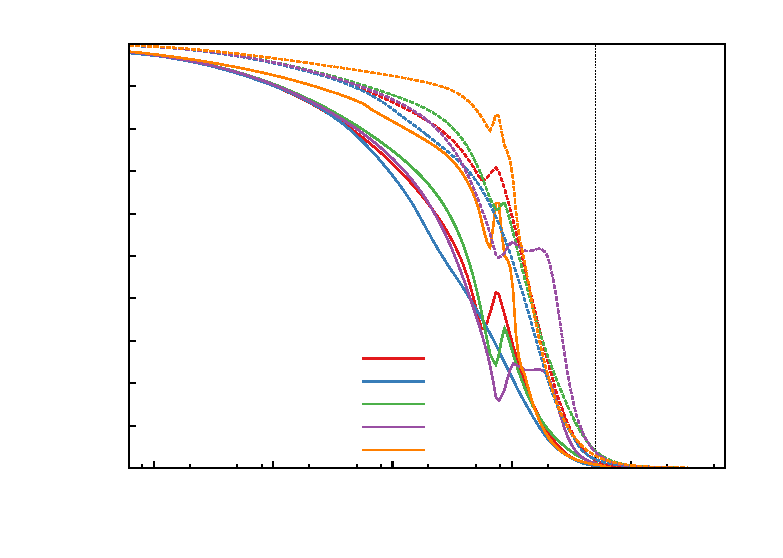
\includegraphics{images/delta-pressure-vs-density}}%
    \gplfronttext
  \end{picture}%
\endgroup

%	\caption[Difference in pressure vs. density for constant $Y_e$, varying temperature]{
%		Normalized pressure difference at $Y_e = 0.05$ between $T = (0,5) {\rm MeV}$ (solid) and $T = (0,10) {\rm MeV}$ (dashed), both normalized by the zero-temperature pressure. Vertical dotted line represents the fiducial density.
%	}
%	\label{fig:dPvsRho}
%\end{figure}


%\begin{figure}
%	\centering
%	% GNUPLOT: LaTeX picture with Postscript
\begingroup
\newcommand{\ft}[0]{\footnotesize}
  \makeatletter
  \providecommand\color[2][]{%
    \GenericError{(gnuplot) \space\space\space\@spaces}{%
      Package color not loaded in conjunction with
      terminal option `colourtext'%
    }{See the gnuplot documentation for explanation.%
    }{Either use 'blacktext' in gnuplot or load the package
      color.sty in LaTeX.}%
    \renewcommand\color[2][]{}%
  }%
  \providecommand\includegraphics[2][]{%
    \GenericError{(gnuplot) \space\space\space\@spaces}{%
      Package graphicx or graphics not loaded%
    }{See the gnuplot documentation for explanation.%
    }{The gnuplot epslatex terminal needs graphicx.sty or graphics.sty.}%
    \renewcommand\includegraphics[2][]{}%
  }%
  \providecommand\rotatebox[2]{#2}%
  \@ifundefined{ifGPcolor}{%
    \newif\ifGPcolor
    \GPcolortrue
  }{}%
  \@ifundefined{ifGPblacktext}{%
    \newif\ifGPblacktext
    \GPblacktexttrue
  }{}%
  % define a \g@addto@macro without @ in the name:
  \let\gplgaddtomacro\g@addto@macro
  % define empty templates for all commands taking text:
  \gdef\gplbacktext{}%
  \gdef\gplfronttext{}%
  \makeatother
  \ifGPblacktext
    % no textcolor at all
    \def\colorrgb#1{}%
    \def\colorgray#1{}%
  \else
    % gray or color?
    \ifGPcolor
      \def\colorrgb#1{\color[rgb]{#1}}%
      \def\colorgray#1{\color[gray]{#1}}%
      \expandafter\def\csname LTw\endcsname{\color{white}}%
      \expandafter\def\csname LTb\endcsname{\color{black}}%
      \expandafter\def\csname LTa\endcsname{\color{black}}%
      \expandafter\def\csname LT0\endcsname{\color[rgb]{1,0,0}}%
      \expandafter\def\csname LT1\endcsname{\color[rgb]{0,1,0}}%
      \expandafter\def\csname LT2\endcsname{\color[rgb]{0,0,1}}%
      \expandafter\def\csname LT3\endcsname{\color[rgb]{1,0,1}}%
      \expandafter\def\csname LT4\endcsname{\color[rgb]{0,1,1}}%
      \expandafter\def\csname LT5\endcsname{\color[rgb]{1,1,0}}%
      \expandafter\def\csname LT6\endcsname{\color[rgb]{0,0,0}}%
      \expandafter\def\csname LT7\endcsname{\color[rgb]{1,0.3,0}}%
      \expandafter\def\csname LT8\endcsname{\color[rgb]{0.5,0.5,0.5}}%
    \else
      % gray
      \def\colorrgb#1{\color{black}}%
      \def\colorgray#1{\color[gray]{#1}}%
      \expandafter\def\csname LTw\endcsname{\color{white}}%
      \expandafter\def\csname LTb\endcsname{\color{black}}%
      \expandafter\def\csname LTa\endcsname{\color{black}}%
      \expandafter\def\csname LT0\endcsname{\color{black}}%
      \expandafter\def\csname LT1\endcsname{\color{black}}%
      \expandafter\def\csname LT2\endcsname{\color{black}}%
      \expandafter\def\csname LT3\endcsname{\color{black}}%
      \expandafter\def\csname LT4\endcsname{\color{black}}%
      \expandafter\def\csname LT5\endcsname{\color{black}}%
      \expandafter\def\csname LT6\endcsname{\color{black}}%
      \expandafter\def\csname LT7\endcsname{\color{black}}%
      \expandafter\def\csname LT8\endcsname{\color{black}}%
    \fi
  \fi
  \setlength{\unitlength}{0.0500bp}%
  \begin{picture}(7200.00,5040.00)%
    \gplgaddtomacro\gplbacktext{%
      \csname LTb\endcsname%
      \put(682,704){\makebox(0,0)[r]{\strut{} 0}}%
      \put(682,1518){\makebox(0,0)[r]{\strut{} 1}}%
      \put(682,2332){\makebox(0,0)[r]{\strut{} 2}}%
      \put(682,3147){\makebox(0,0)[r]{\strut{} 3}}%
      \put(682,3961){\makebox(0,0)[r]{\strut{} 4}}%
      \put(682,4775){\makebox(0,0)[r]{\strut{} 5}}%
      \put(1065,484){\makebox(0,0){\strut{} 1e+11}}%
      \put(2263,484){\makebox(0,0){\strut{} 1e+12}}%
      \put(3460,484){\makebox(0,0){\strut{} 1e+13}}%
      \put(4658,484){\makebox(0,0){\strut{} 1e+14}}%
      \put(5856,484){\makebox(0,0){\strut{} 1e+15}}%
      \put(176,2739){\rotatebox{-270}{\makebox(0,0){\strut{}$\tilde{\Gamma}$}}}%
      \put(3808,154){\makebox(0,0){\strut{}Density (g/cm$^3$)}}%
    }%
    \gplgaddtomacro\gplfronttext{%
      \csname LTb\endcsname%
      \put(1801,4602){\makebox(0,0)[l]{\strut{}Hempel DD2}}%
      \csname LTb\endcsname%
      \put(1801,4382){\makebox(0,0)[l]{\strut{}G. Shen FSU 2.1}}%
      \csname LTb\endcsname%
      \put(1801,4162){\makebox(0,0)[l]{\strut{}SFHo}}%
      \csname LTb\endcsname%
      \put(1801,3942){\makebox(0,0)[l]{\strut{}SFHx}}%
      \csname LTb\endcsname%
      \put(1801,3722){\makebox(0,0)[l]{\strut{}LS220}}%
    }%
    \gplbacktext
    \put(0,0){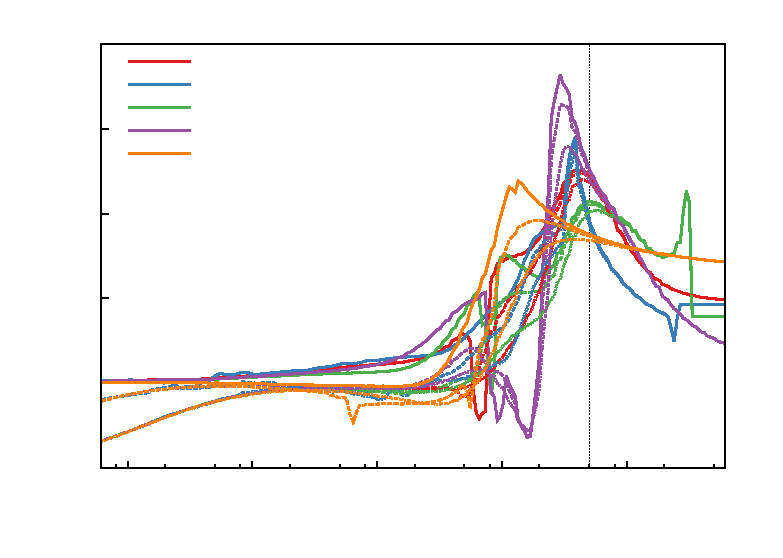
\includegraphics{images/gamma-vs-density}}%
    \gplfronttext
  \end{picture}%
\endgroup

%	\caption[Adiabatic index vs. density for constant $Y_e$, varying temperature]
%	{
%	}
%	\label{fig:GammavsRho}
%\end{figure}


In Figure \ref{fig:MultGammavsRho}, we observe the effect temperature has on the pressure-density relations.  Past the fiducial density $\rho_s = 10^{14.7} {\rm g \, cm^{-3}}$ (with fixed $Y_e = 0.05$), changes in temperature up to $10$MeV do not alter the pressure-density relation by much at all.  As temperature increases in the lower density regime, the structures begin to converge and increase to similar $\tilde{\Gamma}$ between models.  The main differences occur in the intermediate region, where the increasing variance in $\tilde{\Gamma}$ between temperatures becomes clear.

\begin{figure}
	\centering
	% GNUPLOT: LaTeX picture with Postscript
\begingroup
  \makeatletter
  \providecommand\color[2][]{%
    \GenericError{(gnuplot) \space\space\space\@spaces}{%
      Package color not loaded in conjunction with
      terminal option `colourtext'%
    }{See the gnuplot documentation for explanation.%
    }{Either use 'blacktext' in gnuplot or load the package
      color.sty in LaTeX.}%
    \renewcommand\color[2][]{}%
  }%
  \providecommand\includegraphics[2][]{%
    \GenericError{(gnuplot) \space\space\space\@spaces}{%
      Package graphicx or graphics not loaded%
    }{See the gnuplot documentation for explanation.%
    }{The gnuplot epslatex terminal needs graphicx.sty or graphics.sty.}%
    \renewcommand\includegraphics[2][]{}%
  }%
  \providecommand\rotatebox[2]{#2}%
  \@ifundefined{ifGPcolor}{%
    \newif\ifGPcolor
    \GPcolortrue
  }{}%
  \@ifundefined{ifGPblacktext}{%
    \newif\ifGPblacktext
    \GPblacktexttrue
  }{}%
  % define a \g@addto@macro without @ in the name:
  \let\gplgaddtomacro\g@addto@macro
  % define empty templates for all commands taking text:
  \gdef\gplbacktext{}%
  \gdef\gplfronttext{}%
  \makeatother
  \ifGPblacktext
    % no textcolor at all
    \def\colorrgb#1{}%
    \def\colorgray#1{}%
  \else
    % gray or color?
    \ifGPcolor
      \def\colorrgb#1{\color[rgb]{#1}}%
      \def\colorgray#1{\color[gray]{#1}}%
      \expandafter\def\csname LTw\endcsname{\color{white}}%
      \expandafter\def\csname LTb\endcsname{\color{black}}%
      \expandafter\def\csname LTa\endcsname{\color{black}}%
      \expandafter\def\csname LT0\endcsname{\color[rgb]{1,0,0}}%
      \expandafter\def\csname LT1\endcsname{\color[rgb]{0,1,0}}%
      \expandafter\def\csname LT2\endcsname{\color[rgb]{0,0,1}}%
      \expandafter\def\csname LT3\endcsname{\color[rgb]{1,0,1}}%
      \expandafter\def\csname LT4\endcsname{\color[rgb]{0,1,1}}%
      \expandafter\def\csname LT5\endcsname{\color[rgb]{1,1,0}}%
      \expandafter\def\csname LT6\endcsname{\color[rgb]{0,0,0}}%
      \expandafter\def\csname LT7\endcsname{\color[rgb]{1,0.3,0}}%
      \expandafter\def\csname LT8\endcsname{\color[rgb]{0.5,0.5,0.5}}%
    \else
      % gray
      \def\colorrgb#1{\color{black}}%
      \def\colorgray#1{\color[gray]{#1}}%
      \expandafter\def\csname LTw\endcsname{\color{white}}%
      \expandafter\def\csname LTb\endcsname{\color{black}}%
      \expandafter\def\csname LTa\endcsname{\color{black}}%
      \expandafter\def\csname LT0\endcsname{\color{black}}%
      \expandafter\def\csname LT1\endcsname{\color{black}}%
      \expandafter\def\csname LT2\endcsname{\color{black}}%
      \expandafter\def\csname LT3\endcsname{\color{black}}%
      \expandafter\def\csname LT4\endcsname{\color{black}}%
      \expandafter\def\csname LT5\endcsname{\color{black}}%
      \expandafter\def\csname LT6\endcsname{\color{black}}%
      \expandafter\def\csname LT7\endcsname{\color{black}}%
      \expandafter\def\csname LT8\endcsname{\color{black}}%
    \fi
  \fi
  \setlength{\unitlength}{0.0500bp}%
  \begin{picture}(7200.00,5040.00)%
    \gplgaddtomacro\gplbacktext{%
      \csname LTb\endcsname%
      \put(682,704){\makebox(0,0)[r]{\strut{} 0}}%
      \put(682,1518){\makebox(0,0)[r]{\strut{} 1}}%
      \put(682,2332){\makebox(0,0)[r]{\strut{} 2}}%
      \put(682,3147){\makebox(0,0)[r]{\strut{} 3}}%
      \put(682,3961){\makebox(0,0)[r]{\strut{} 4}}%
      \put(682,4775){\makebox(0,0)[r]{\strut{} 5}}%
      \put(1065,484){\makebox(0,0){\strut{} 1e+11}}%
      \put(2263,484){\makebox(0,0){\strut{} 1e+12}}%
      \put(3460,484){\makebox(0,0){\strut{} 1e+13}}%
      \put(4658,484){\makebox(0,0){\strut{} 1e+14}}%
      \put(5856,484){\makebox(0,0){\strut{} 1e+15}}%
      \put(176,2739){\rotatebox{-270}{\makebox(0,0){\strut{}$\tilde{\Gamma}$}}}%
      \put(3808,154){\makebox(0,0){\strut{}Density (g/cm$^3$)}}%
      \put(5613,3961){\rotatebox{90}{\makebox(0,0)[l]{\strut{}\small $\rho_{\rm fid}$}}}%
    }%
    \gplgaddtomacro\gplfronttext{%
      \csname LTb\endcsname%
      \put(1801,4602){\makebox(0,0)[l]{\strut{}Hempel DD2}}%
      \csname LTb\endcsname%
      \put(1801,4382){\makebox(0,0)[l]{\strut{}G. Shen FSU 2.1}}%
      \csname LTb\endcsname%
      \put(1801,4162){\makebox(0,0)[l]{\strut{}SFHo}}%
      \csname LTb\endcsname%
      \put(1801,3942){\makebox(0,0)[l]{\strut{}SFHx}}%
      \csname LTb\endcsname%
      \put(1801,3722){\makebox(0,0)[l]{\strut{}LS220}}%
      \csname LTb\endcsname%
      \put(5025,3961){\rotatebox{90}{\makebox(0,0)[l]{\strut{}\small $\rho_{\rm sat}$}}}%
      \put(5857,1635){\makebox(0,0)[l]{\strut{}\small $\tilde{\Gamma} = 4/3$}}%
    }%
    \gplbacktext
    \put(0,0){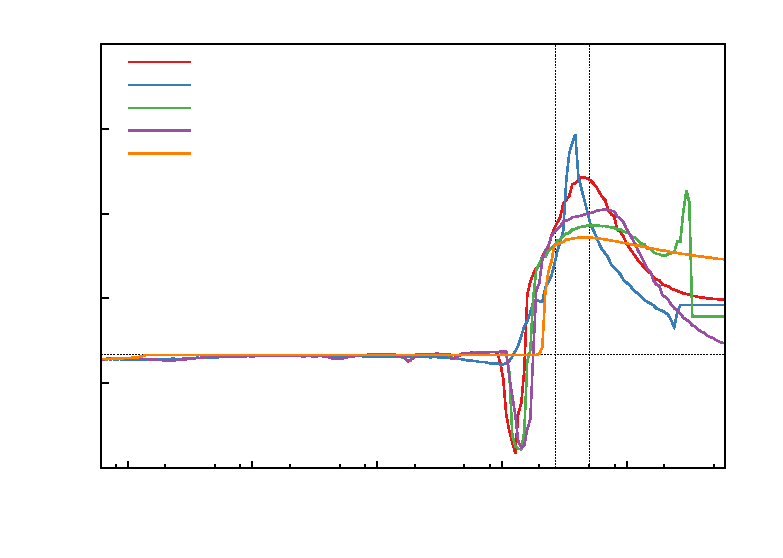
\includegraphics{images/one-gamma-vs-density}}%
    \gplfronttext
  \end{picture}%
\endgroup

	\caption[Adiabatic index vs. density for constant composition and temperature]
	{
		Effective adiabatic index as a function of baryon density for constant $Y_e = 0.3$ and temperature $T = 0.7 {\rm MeV}$, for comparison to the literature~\cite{Fischer2014}.  Displayed are vertical lines for the critical density $\rho_c$ and fiducial density $\rho_{\rm fid}$, while the third vertical line to the right is the nuclear saturation density.  The horizontal line corresponds to a $\Gamma = 4/3$ polytrope law.
	}
	\label{fig:OneGammavsRho}
\end{figure}


\begin{figure}[]
	\centering
	\footnotesize{	
		% GNUPLOT: LaTeX picture with Postscript
\begingroup
\newcommand{\ft}[0]{\footnotesize}
  \makeatletter
  \providecommand\color[2][]{%
    \GenericError{(gnuplot) \space\space\space\@spaces}{%
      Package color not loaded in conjunction with
      terminal option `colourtext'%
    }{See the gnuplot documentation for explanation.%
    }{Either use 'blacktext' in gnuplot or load the package
      color.sty in LaTeX.}%
    \renewcommand\color[2][]{}%
  }%
  \providecommand\includegraphics[2][]{%
    \GenericError{(gnuplot) \space\space\space\@spaces}{%
      Package graphicx or graphics not loaded%
    }{See the gnuplot documentation for explanation.%
    }{The gnuplot epslatex terminal needs graphicx.sty or graphics.sty.}%
    \renewcommand\includegraphics[2][]{}%
  }%
  \providecommand\rotatebox[2]{#2}%
  \@ifundefined{ifGPcolor}{%
    \newif\ifGPcolor
    \GPcolortrue
  }{}%
  \@ifundefined{ifGPblacktext}{%
    \newif\ifGPblacktext
    \GPblacktexttrue
  }{}%
  % define a \g@addto@macro without @ in the name:
  \let\gplgaddtomacro\g@addto@macro
  % define empty templates for all commands taking text:
  \gdef\gplbacktext{}%
  \gdef\gplfronttext{}%
  \makeatother
  \ifGPblacktext
    % no textcolor at all
    \def\colorrgb#1{}%
    \def\colorgray#1{}%
  \else
    % gray or color?
    \ifGPcolor
      \def\colorrgb#1{\color[rgb]{#1}}%
      \def\colorgray#1{\color[gray]{#1}}%
      \expandafter\def\csname LTw\endcsname{\color{white}}%
      \expandafter\def\csname LTb\endcsname{\color{black}}%
      \expandafter\def\csname LTa\endcsname{\color{black}}%
      \expandafter\def\csname LT0\endcsname{\color[rgb]{1,0,0}}%
      \expandafter\def\csname LT1\endcsname{\color[rgb]{0,1,0}}%
      \expandafter\def\csname LT2\endcsname{\color[rgb]{0,0,1}}%
      \expandafter\def\csname LT3\endcsname{\color[rgb]{1,0,1}}%
      \expandafter\def\csname LT4\endcsname{\color[rgb]{0,1,1}}%
      \expandafter\def\csname LT5\endcsname{\color[rgb]{1,1,0}}%
      \expandafter\def\csname LT6\endcsname{\color[rgb]{0,0,0}}%
      \expandafter\def\csname LT7\endcsname{\color[rgb]{1,0.3,0}}%
      \expandafter\def\csname LT8\endcsname{\color[rgb]{0.5,0.5,0.5}}%
    \else
      % gray
      \def\colorrgb#1{\color{black}}%
      \def\colorgray#1{\color[gray]{#1}}%
      \expandafter\def\csname LTw\endcsname{\color{white}}%
      \expandafter\def\csname LTb\endcsname{\color{black}}%
      \expandafter\def\csname LTa\endcsname{\color{black}}%
      \expandafter\def\csname LT0\endcsname{\color{black}}%
      \expandafter\def\csname LT1\endcsname{\color{black}}%
      \expandafter\def\csname LT2\endcsname{\color{black}}%
      \expandafter\def\csname LT3\endcsname{\color{black}}%
      \expandafter\def\csname LT4\endcsname{\color{black}}%
      \expandafter\def\csname LT5\endcsname{\color{black}}%
      \expandafter\def\csname LT6\endcsname{\color{black}}%
      \expandafter\def\csname LT7\endcsname{\color{black}}%
      \expandafter\def\csname LT8\endcsname{\color{black}}%
    \fi
  \fi
  \setlength{\unitlength}{0.0500bp}%
  \begin{picture}(8640.00,6552.00)%
    \gplgaddtomacro\gplbacktext{%
      \csname LTb\endcsname%
      \put(732,3276){\makebox(0,0)[r]{\strut{}0}}%
      \put(732,3822){\makebox(0,0)[r]{\strut{}1}}%
      \put(732,4367){\makebox(0,0)[r]{\strut{}2}}%
      \put(732,4913){\makebox(0,0)[r]{\strut{}3}}%
      \put(732,5459){\makebox(0,0)[r]{\strut{}4}}%
      \put(1009,3056){\makebox(0,0){\strut{}}}%
      \put(1700,3056){\makebox(0,0){\strut{}}}%
      \put(2391,3056){\makebox(0,0){\strut{}}}%
      \put(3082,3056){\makebox(0,0){\strut{}}}%
      \put(3773,3056){\makebox(0,0){\strut{}}}%
      \put(4043,5633){\makebox(0,0)[l]{\strut{}a}}%
    }%
    \gplgaddtomacro\gplfronttext{%
      \csname LTb\endcsname%
      \put(1851,5722){\makebox(0,0)[l]{\strut{}Hempel DD2}}%
      \csname LTb\endcsname%
      \put(1851,5502){\makebox(0,0)[l]{\strut{}G. Shen FSU 2.1}}%
      \csname LTb\endcsname%
      \put(1851,5282){\makebox(0,0)[l]{\strut{}SFHo}}%
      \csname LTb\endcsname%
      \put(1851,5062){\makebox(0,0)[l]{\strut{}SFHx}}%
      \csname LTb\endcsname%
      \put(1851,4842){\makebox(0,0)[l]{\strut{}LS220}}%
    }%
    \gplgaddtomacro\gplbacktext{%
      \csname LTb\endcsname%
      \put(4188,3276){\makebox(0,0)[r]{\strut{}}}%
      \put(4188,3822){\makebox(0,0)[r]{\strut{}}}%
      \put(4188,4367){\makebox(0,0)[r]{\strut{}}}%
      \put(4188,4913){\makebox(0,0)[r]{\strut{}}}%
      \put(4188,5459){\makebox(0,0)[r]{\strut{}}}%
      \put(4465,3056){\makebox(0,0){\strut{}}}%
      \put(5156,3056){\makebox(0,0){\strut{}}}%
      \put(5847,3056){\makebox(0,0){\strut{}}}%
      \put(6538,3056){\makebox(0,0){\strut{}}}%
      \put(7229,3056){\makebox(0,0){\strut{}}}%
      \put(7499,5633){\makebox(0,0)[l]{\strut{}b}}%
    }%
    \gplgaddtomacro\gplfronttext{%
    }%
    \gplgaddtomacro\gplbacktext{%
      \csname LTb\endcsname%
      \put(732,655){\makebox(0,0)[r]{\strut{}0}}%
      \put(732,1201){\makebox(0,0)[r]{\strut{}1}}%
      \put(732,1747){\makebox(0,0)[r]{\strut{}2}}%
      \put(732,2293){\makebox(0,0)[r]{\strut{}3}}%
      \put(732,2838){\makebox(0,0)[r]{\strut{}4}}%
      \put(1009,435){\makebox(0,0){\strut{} 1e+11}}%
      \put(1700,435){\makebox(0,0){\strut{} 1e+12}}%
      \put(2391,435){\makebox(0,0){\strut{} 1e+13}}%
      \put(3082,435){\makebox(0,0){\strut{} 1e+14}}%
      \put(3773,435){\makebox(0,0){\strut{} 1e+15}}%
      \put(4043,3013){\makebox(0,0)[l]{\strut{}c}}%
    }%
    \gplgaddtomacro\gplfronttext{%
    }%
    \gplgaddtomacro\gplbacktext{%
      \csname LTb\endcsname%
      \put(4188,655){\makebox(0,0)[r]{\strut{}}}%
      \put(4188,1201){\makebox(0,0)[r]{\strut{}}}%
      \put(4188,1747){\makebox(0,0)[r]{\strut{}}}%
      \put(4188,2293){\makebox(0,0)[r]{\strut{}}}%
      \put(4188,2838){\makebox(0,0)[r]{\strut{}}}%
      \put(4465,435){\makebox(0,0){\strut{} 1e+11}}%
      \put(5156,435){\makebox(0,0){\strut{} 1e+12}}%
      \put(5847,435){\makebox(0,0){\strut{} 1e+13}}%
      \put(6538,435){\makebox(0,0){\strut{} 1e+14}}%
      \put(7229,435){\makebox(0,0){\strut{} 1e+15}}%
      \put(491,3275){\rotatebox{-270}{\makebox(0,0){\strut{}$\tilde{\Gamma}$}}}%
      \put(4319,105){\makebox(0,0){\strut{}$\rho_0$ (g/cm$^3$)}}%
      \put(7499,3013){\makebox(0,0)[l]{\strut{}d}}%
    }%
    \gplgaddtomacro\gplfronttext{%
    }%
    \gplbacktext
    \put(0,0){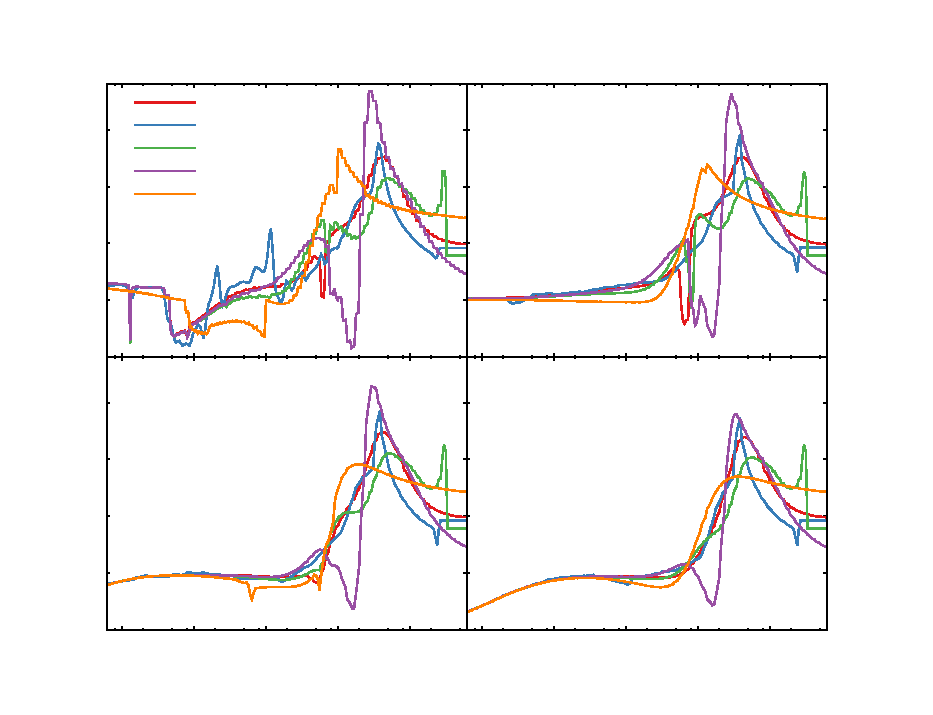
\includegraphics{images/mp-gamma-vs-density}}%
    \gplfronttext
  \end{picture}%
\endgroup

	}
	\caption[Adiabatic index vs. density for constant $Y_e = 0.3$, varying temperature]
	{
		Effective adiabatic index as a function of density for the equaions of state considered, sliced along 
		(a) cold $T=0.1 {\rm MeV}$, $\beta$-equilibrium,
		(b) temperature $T=0 {\rm MeV}$,
		(c) $T=5{\rm MeV}$,
		(d) $T=10{\rm MeV}$,
		where cases (b)-(d) also assume very neutron rich composition $Y_e = 0.05$.  In all models, as atmosphere temperature increases the equations of state all begin to soften and become less distinguishable.  
		The step-effect in (a) is likely the result of a low resolution used in the $\beta$-equilibrium slice. 
	}
	\label{fig:MultGammavsRho}
\end{figure}
